\documentclass{report}

\input{~/dev/latex/template/preamble.tex}
\input{~/dev/latex/template/macros.tex}

\title{\Huge{}}
\author{\huge{Nathan Warner}}
\date{\huge{}}
\pagestyle{fancy}
\fancyhf{}
\lhead{Warner \thepage}
\rhead{}
% \lhead{\leftmark}
\cfoot{\thepage}
%\setborder
% \usepackage[default]{sourcecodepro}
% \usepackage[T1]{fontenc}

\begin{document}
    % \maketitle
        \begin{titlepage}
       \begin{center}
           \vspace*{1cm}
    
           \textbf{Calculus 2} \\
           Chapter 3
    
           \vspace{0.5cm}
            
                
           \vspace{1.5cm}
    
           \textbf{Nathan Warner}
    
           \vfill
                
                
           \vspace{0.8cm}
         
           
\includegraphics[width=0.4\textwidth]{~/niu/seal.png}
                
           Computer Science \\
           Northern Illinois University\\
           September 27, 2023 \\
           United States\\
           
                
       \end{center}
    \end{titlepage}
    \tableofcontents
    \pagebreak \bigbreak \noindent
    \vspace{2in} \\
    \begin{Huge}
       \textbf{Techniques of Integration} 
    \end{Huge}
    \bigbreak \noindent 
    \line(1,0){490}
    \bigbreak \noindent 
    
    \phantomsection
    \addcontentsline{toc}{section}{\Large 3.1 Integration by Parts}
    \section*{\Large 3.1 Integration by Parts}
    \bigbreak \noindent 
    \smallbreak \noindent
    \begin{definition}
        Many students want to know whether there is a product rule for integration. There isn’t, but there is a technique based on the product rule for differentiation that allows us to exchange one integral for another. We call this technique \textbf{integration by parts.}
    \end{definition}

    \bigbreak \noindent 
    \phantomsection
    \addcontentsline{toc}{subsection}{The Integration-by-Parts Formula}
    \subsection*{The Integration-by-Parts Formula}
    \bigbreak \noindent 
    If, \( h(x) = f(x)g(x) \),
then by using the product rule, we obtain \( h'(x) = f'(x)g(x) + g'(x)f(x) \).
Although at first it may seem counterproductive, let’s now integrate both sides of this equation:
\[ \int h'(x) \, dx = \int \left( g(x)f'(x) + f(x)g'(x) \right) \, dx. \]
\bigbreak \noindent 
This gives us
\[ h(x) = f(x)g(x) = \int g(x)f'(x) \, dx + \int f(x)g'(x) \, dx. \]
Now we solve for \( \int f(x)g'(x) \, dx \):
\[ \int f(x)g'(x) \, dx = f(x)g(x) - \int g(x)f'(x) \, dx. \]
By making the substitutions \( u = f(x) \)
and \( v = g(x) \),
which in turn make \( du = f'(x) \, dx \)
and \( dv = g'(x) \, dx \),
we have the more compact form
\[ \int u \, dv = uv - \int v \, du. \]


    \pagebreak \bigbreak \noindent 
    \begin{thrm}[Integration by Parts]
        Let \( u = f(x) \)  and \( v = g(x) \)  be functions with continuous derivatives. Then, the integration-by-parts formula for the integral involving these two functions is: \[ \int u \, dv = uv - \int v \, du. \]
    \end{thrm}

    \bigbreak \noindent \bigbreak \noindent 
    \begin{eg}[Using Integration by Parts]
        Use integration by parts with \( u = x \)
and \( dv = \sin x \, dx \)
to evaluate 
\[ \int x \sin x \, dx. \]
        
    \end{eg}
    \bigbreak \noindent 
    \pf{Solution}{
        So to use the formula:
        \begin{align*}
            \int_{}^{}\ u\ dv = uv - \int v\ du
        .\end{align*}
        \bigbreak \noindent 
        We need:
        \begin{align*}
            u = x \quad du = dx \\
            dv = \sin{x}dx \quad v = -\cos{x}
        .\end{align*}
        \bigbreak \noindent 
        Thus:
        \begin{align*}
            \int x\sin{x}\ dx &= -x\cos{x} - \int -\cos{x}\ dx \\
                              &=-x\cos{x} + \sin{x} + C
        .\end{align*}
    

    }
    \bigbreak \noindent 
    The natural question to ask at this point is: How do we know how to choose  u
  and  dv?
  Sometimes it is a matter of trial and error; however, the acronym \textbf{LIATE} can often help to take some of the guesswork out of our choices. This acronym stands for 
  \begin{itemize}
      \item \textbf{L}ogarithmic Functions
      \item \textbf{I}nverse Trigonometric Functions
      \item \textbf{A}lgebraic Functions
      \item \textbf{T}rigonometric Functions
        \item \textbf{E}ponential Functions
  \end{itemize}
    This mnemonic serves as an aid in determining an appropriate choice for  u.
    \bigbreak \noindent 
    \nt{A better version might be LIAET, where exponential and trig functions are swapped}

    \pagebreak 
    \phantomsection
    \addcontentsline{toc}{subsection}{Applying integration by parts more than once}
    \subsection*{Applying integration by parts more than once}
    \bigbreak \noindent 
    \begin{eg}[Evaluate]
       \begin{align*}
            \int x^{2}e^{3x}\ dx
       .\end{align*}
    \end{eg}
    \bigbreak \noindent 
    \pf{Solution}{
        By \textbf{LIATE}, we let $u=x^{2}$, and $dv= e^{3x}$. Thus, we get:
        \begin{align*}
            &u=x^{2} \quad dv = e^{3x} \\
            &du=2xdx \quad v = \frac{1}{3}e^{3x}
        .\end{align*}
        \bigbreak \noindent 
        Then by theorem 1, we get:
        \begin{align*}
            \int udv &= uv - \int vdu \\
            &=\int x^{2}e^{3x}\ dx = x^{2}\frac{1}{3}e^{3x} - \int \frac{1}{3}e^{3x}2x\ dx \\
            &=\int x^{2}e^{3x}\ dx = x^{2}\frac{1}{3}e^{3x} - \int \frac{2}{3}e^{3x}x\ dx \\
        .\end{align*}
        \bigbreak \noindent 
        At this point, we will notice that we still cannot evaluate the integral $\int \frac{2}{3}e^{3x}x\ dx $. Thus, we must apply the theorem once more.
        \bigbreak \noindent 
        \begin{minipage}[]{0.47\textwidth}
            \begin{align*}
            &\int \frac{2}{3}e^{3x}x\ dx  \\
            &u = x \quad dv = \frac{2}{3}e^{3x} \\
            &du = dx \quad v = \frac{2}{9}e^{3x}
        .\end{align*}
        \end{minipage}
        \begin{minipage}[]{0.47\textwidth}
            Thus:
            \begin{align*}
                \int \frac{2}{3}e^{3x}\ dx &= \frac{2}{9}e^{3x}x - \int \frac{2}{9}e^{3x}\ dx \\
                                       &=\frac{2}{9}xe^{3x} - \frac{2}{27}e^{3x}
            .\end{align*}
        \end{minipage}
        \bigbreak \noindent 
        In full we have:
        \begin{align*}
            &\int x^{2}e^{3x}\ dx = \frac{1}{3}x^{2}e^{3x} - \left(\frac{2}{9}xe^{3x}-\frac{2}{27}e^{3x}\right) \\
            &=\frac{1}{3}e^{3x}x^{2}-\frac{2}{9}xe^{3x}+\frac{2}{27}e^{3x} + C
        .\end{align*}
    
    }

    \pagebreak 
    \phantomsection
    \addcontentsline{toc}{subsection}{Applying Integration by Parts When LIATE Doesn’t Quite Work}
    \subsection*{Applying Integration by Parts When LIATE Doesn’t Quite Work}
    \bigbreak \noindent 
    \begin{eg}[Evaluate]
        \begin{align*}
            \int t^{3}e^{t^{2}}\ dt
        .\end{align*}
    \end{eg}
    \bigbreak \noindent 
    \pf{Solution}{
        If we use a strict interpretation of the mnemonic \textbf{LIATE} to make our choice of  $u$, we end up with  $u = t^3$  and  $dv = e^{t^2} dt$. 
        Unfortunately, this choice won’t work because we are unable to evaluate  $\int e^{t^2}\ dt$.  However, since we can evaluate  $\int t e^{t^2}\ dt$, we can try choosing  $u = t^2$ and  $dv = t e^{t^2}\ dt$. With these choices we have
        \begin{align*}
            &u = t^{2} \quad dv = te^{t^{2}} \\
            &du = 2t\ dt \quad v = \frac{1}{2}e^{t^{2}}
        .\end{align*}
        \bigbreak \noindent 
        Thus, we obtain:
        \begin{align*}
            \int t^{3}e^{t^{2}}\ dt &= \frac{1}{2}t^{2}e^{t^{2}} - \int \frac{1}{2}e^{t^{2}}2t\\
            &= \frac{1}{2}t^{2}e^{t^{2}} - \int e^{t^{2}}t\ dt \\
            &= \frac{1}{2}t^{2}e^{t^{2}} - \frac{1}{2}e^{t^{2}} + C 
        .\end{align*}

        }

        \bigbreak \noindent 
        \begin{eg}[Evaluate]
            \begin{align*}
                \int \sin{(\ln{(x)})}\ dx
            .\end{align*}
            \bigbreak \noindent 
        \end{eg}
        \pf{Solution}{
            Here, we let $u = \sin{(\ln{(x)})}$ and $dv = 1dx$, so we have:
            \begin{align*}
                &u = \sin{(\ln{(x)})} \quad dv = dx \\
                &du = \frac{1}{x}\cos{(\ln{(x)})}\ dx \quad v = x
            .\end{align*}
            \bigbreak \noindent 
            Which gives us:
            \begin{align*}
                \int \sin{(\ln{(x)})}\ dx = x\sin{(\ln{(x)})} - \int \cos{(\ln{(x)})}\ dx
            .\end{align*}
            \bigbreak \noindent 
            Which leaves us in no better shape than the original integral, so we apply the theorem once more:
            \bigbreak \noindent 
            \begin{minipage}[]{0.47\textwidth}
                \begin{align*}
                    &\int \cos{(\ln{(x)})} \\
                    &u = \cos{(\ln{(x)})} \quad dv = dx \\
                    &du = -\frac{1}{x}\sin{(\ln{(x)})}\ dx \quad v = x
                .\end{align*}
            \end{minipage}
            \begin{minipage}[]{0.47\textwidth}
                Thus we have:
                \begin{align*}
                    \int \cos{(\ln{(x)})} &= x\cos{(\ln{(x)})} - \int -\sin{(\ln{(x)})}\ dx
                .\end{align*}
            \end{minipage}
            \bigbreak \noindent 
            At this point, we have:
            \begin{align*}
                \int \sin{(\ln{(x)})}\ dx &= x\sin{(\ln{(x)})} - \left(x\cos{(\ln{(x)})}- \int -\sin{(ln(x))}\ dx\right) \\
                &= x\sin{(\ln{(x)})} - \left(x\cos{(\ln{(x)})}+ \int \sin{(ln(x))}\ dx\right) \\
                &= x\sin{(\ln{(x)})} - x\cos{(\ln{(x)})}- \int \sin{(ln(x))}\ dx \\
            .\end{align*}
            \bigbreak \noindent 
            The last integral is now the same as the original. It may seem that we have simply gone in a circle, but now we can actually evaluate the integral. To see how to do this more clearly, substitute:
            \begin{align*}
                I = \int \sin{(\ln{(x)})}\ dx
            .\end{align*}
            \bigbreak \noindent 
            Thus, the equation becomes:
            \begin{align*}
                I &= x\sin{(\ln{(x)})} - x\cos{(\ln{(x)})} - I \\
                  2I&=x\sin{(\ln{(x)})} - x\cos{(\ln{(x)})}  \\
                    I&= \frac{1}{2}x\sin{(\ln{(x)})} - \frac{1}{2}x\cos{(\ln{(x)})}
            .\end{align*}
            \bigbreak \noindent 
            Substituting back in for $I$ we get:
            \begin{align*}
                \int \sin{(\ln{(x)})}\ dx  = \frac{1}{2}x\sin{(\ln{(x)})} - \frac{1}{2}x\cos{(\ln{(x)})} + C
            .\end{align*}
            \bigbreak \noindent 
        }

        \bigbreak \noindent 
        \phantomsection
        \addcontentsline{toc}{subsection}{Integration by parts for definite integrals}
        \subsection*{Integration by parts for definite integrals}
        \bigbreak \noindent 
        Now that we have used integration by parts successfully to evaluate indefinite integrals, we turn our attention to definite integrals. The integration technique is really the same, only we add a step to evaluate the integral at the upper and lower limits of integration.
        \bigbreak \noindent 
        \begin{thrm}[Integration by Parts for Definite Integrals]
           Let  $u = f(x)$  and  $v = g(x)$ be functions with continuous derivatives on $[a,b]$. Then:
           \begin{align*}
               \int_{a}^{b} u \, dv &= uv\big|_{a}^{b} - \int_{a}^{b} v \, du
           .\end{align*}
        \end{thrm}

        \pagebreak 
        \phantomsection
        \addcontentsline{toc}{section}{3.2 Trigonometric Integrals}
        \section*{3.2 Trigonometric Integrals}
        \bigbreak \noindent 
        In this section we look at how to integrate a variety of products of trigonometric functions. These integrals are called trigonometric integrals. They are an important part of the integration technique called trigonometric substitution, which is featured in Trigonometric Substitution. This technique allows us to convert algebraic expressions that we may not be able to integrate into expressions involving trigonometric functions, which we may be able to integrate using the techniques described in this section. In addition, these types of integrals appear frequently when we study polar, cylindrical, and spherical coordinate systems later. Let’s begin our study with products of $\sin{x}$ and $\cos{x}$.

        \bigbreak \noindent 
        \begin{large}
            \textbf{Integrating $\cos^{j}{x}\sin{x}$}
        \end{large}
        \bigbreak \noindent 
        In this case, we can preform a simple u-substation, where we let $u=\cos{x}$, and from there we can evaluate.
        \bigbreak \noindent 
        \begin{eg}[Evaluate]
           \begin{align*}
               &\int \cos^{5}{x}\sin{x}\ dx \\
               &=- \int u^{5}\ du \\
               &-\frac{1}{6}u^{6} + C \\
               &= -\frac{1}{6}\cos^{6}{x} + C
           .\end{align*} 
        \end{eg}
        
        \bigbreak \noindent 
        \begin{large}
            \textbf{Integrating $\cos^{j}{x}\sin^{k}{x}$ when $k$ is odd}
        \end{large}
        \bigbreak \noindent 
        In this case, we can use the trigonometric identity: $\sin^{2}{x} = 1-\cos^{2}{x}$ to rewrite the expression such that using a u-substation will work. In general:
        \begin{align*}
            &\int \cos^{j}{x}\sin^{k}{x}\ dx\quad \text{s.t}\ k = 2l+1\ l \in \mathbb{Z} \\
            &=\int \cos^{j}{x}(1-\cos^{2}{k})^{\frac{k-1}{2}}\sin{(x)}
        .\end{align*}
        \bigbreak \noindent 
        \begin{eg}[Evaluate]
            \begin{align*}
                &\int \cos^{2}{x}\sin^{5}{x}\ dx \\
                &=\int\cos^{2}{x}(1-\cos^{2}{x})^{\frac{5-1}{2}}\sin{x}\ dx \\
                &=\int \cos^{2}{x}(1-\cos^{2}{x})^{2}\sin{x}\ dx \\
                &=etc...
            .\end{align*}
        \end{eg}
        \bigbreak \noindent 
        \nt{This fact also holds for $\int \sin^{j}{x}\cos^{k}{x}\, for\ k = 2l+1,\ l \in \mathbb{Z}$}

        \pagebreak 
        \phantomsection
        \addcontentsline{toc}{subsection}{Integrating even powers of sin(x)}
        \subsection*{Integrating even powers of $\sin{x}$}
        \bigbreak \noindent 
        In the next example, we see the strategy that must be applied when there are only even powers of \( \sin(x) \) and \( \cos(x) \). For integrals of this type, the identities
        \[
        \sin^2(x) = \frac{1}{2} - \frac{1}{2}\cos(2x) = \frac{1 - \cos(2x)}{2}
        \]
        and
        \[
        \cos^2(x) = \frac{1}{2} + \frac{1}{2}\cos(2x) = \frac{1 + \cos(2x)}{2}
        \]
        are invaluable. These identities are sometimes known as power-reducing identities and they may be derived from the double-angle identity  $\cos(2x) = \cos^2(x) - \sin^2(x)$ and the Pythagorean identity  $\cos^2(x) + \sin^2(x) = 1$

        \bigbreak \noindent 
        \begin{eg}[Evaluate]
           \begin{align*}
               &\int \sin^{2}{x}\ dx
           .\end{align*} 
           \bigbreak \noindent 
           By the identity described above, we can derive:
           \begin{align*}
               \cos{2x} &= 1-2\sin^{2}{x} \\
               \sin^{2}{x} &= \frac{1}{2}-\frac{1}{2}\cos{2x} 
           .\end{align*}
           \bigbreak \noindent 
           Thus we have:
           \begin{align*}
               &\int \frac{1}{2}-\frac{1}{2}\cos{2x}\ dx \\
               &=\frac{1}{2}x - \frac{1}{4}\sin{2x} + C
           .\end{align*}
        \end{eg}

        \pagebreak 
        \phantomsection
        \addcontentsline{toc}{subsection}{Problem-Solving Strategy: Integrating Products and Powers of sin x and cos x}
        \subsection*{Problem-Solving Strategy: Integrating Products and Powers of sin x and cos x}
        \bigbreak \noindent 
        To integrate 
\[
\int \cos^j(x) \sin^k(x) \, dx
\]
use the following strategies:

\begin{enumerate}
    \item If \( k \) is odd, rewrite \( \sin^k(x) \) as \( \sin^{k-1}(x) \sin(x) \) and use the identity \( \sin^2(x) = 1 - \cos^2(x) \) to rewrite \( \sin^{k-1}(x) \) in terms of \( \cos(x) \). Integrate using the substitution \( u = \cos(x) \). This substitution makes \( du = -\sin(x) \, dx \).
    
    \item If \( j \) is odd, rewrite \( \cos^j(x) \) as \( \cos^{j-1}(x) \cos(x) \) and use the identity \( \cos^2(x) = 1 - \sin^2(x) \) to rewrite \( \cos^{j-1}(x) \) in terms of \( \sin(x) \). Integrate using the substitution \( u = \sin(x) \). This substitution makes \( du = \cos(x) \, dx \). (Note: If both \( j \) and \( k \) are odd, either strategy 1 or strategy 2 may be used.)
    
    \item If both \( j \) and \( k \) are even, use 
    \[
    \sin^2(x) = \frac{1}{2} - \frac{1}{2} \cos(2x)
    \]
    and 
    \[
    \cos^2(x) = \frac{1}{2} + \frac{1}{2} \cos(2x).
    \]
    After applying these formulas, simplify and reapply strategies 1 through 3 as appropriate.
\end{enumerate}

    \bigbreak \noindent 
    \phantomsection
    \addcontentsline{toc}{subsection}{Power reduction formulas}
    \subsection*{Power reduction formulas}
    \bigbreak \noindent 
    \begin{thrm}[Power reduction formulas]
        \begin{itemize}
            \item \textbf{Power Reduction Formula (sine)}
                \begin{align*}
                    \int \sin^{n}{x}\ dx = -\frac{1}{n}\sin^{n-1}{x}\cos{x} + \frac{n-1}{n}\int \sin^{n-2}{x}\ dx
                .\end{align*}
            \item \textbf{Power Reduction Formula (cosine)}
                \begin{align*}
                    \int \cos^{n}{x}\ dx = \frac{1}{n}\cos^{n-1}{x}\sin{x} + \frac{n-1}{n}\int \cos^{n-2}{x}\ dx
                .\end{align*}
            \item \textbf{Power Reduction Formula (secant)}
            \begin{align*}
                \int \sec^{n}{x}\ dx &= \frac{1}{n-1}\sec^{n-1}{x}\sin{x}+\frac{n-2}{n-1}\int \sec^{n-2}{x}\ dx \\
                \int \sec^{n}{x}\ dx &= \frac{1}{n-1}\sec^{n-2}{x}\tan{x}+\frac{n-2}{n-1}\int \sec^{n-2}{x}\ dx
            \end{align*}
            \item \textbf{Power Reduction Formula (Tangent)}
                \begin{align*}
                    \int \tan^{n}{x}\ dx &= \frac{1}{n-1}\tan^{n-1}{x} - \int \tan^{n-2}{x}\ dx
                .\end{align*}
        \end{itemize}
    \end{thrm}
    

    \pagebreak 
    \phantomsection
    \addcontentsline{toc}{subsection}{Integrating products of sines and cosines of different angles}
    \subsection*{Integrating products of sines and cosines of different angles}
    \bigbreak \noindent 
    \begin{thrm}
       To integrate products involving  sin(ax), sin(bx), cos(ax), and  cos(bx), use the substitutions:
       \begin{itemize}
           \item \textbf{Sine Products}
            \begin{align*}
                \sin(ax) \sin(bx) &= \frac{1}{2} \cos((a-b)x) - \frac{1}{2} \cos((a+b)x)
            \end{align*}

            \item \textbf{Sine and Cosine Products}
            \begin{align*}
                \sin(ax) \cos(bx) &= \frac{1}{2} \sin((a-b)x) + \frac{1}{2} \sin((a+b)x)
            \end{align*}

            \item \textbf{Cosine Products}
            \begin{align*}
                \cos(ax) \cos(bx) &= \frac{1}{2} \cos((a-b)x) + \frac{1}{2} \cos((a+b)x)
            \end{align*}
       \end{itemize}
       \bigbreak \noindent 
       Which are trivial if you know the trigonometric \textbf{product to sum} identities
    \end{thrm}

    \pagebreak 
    \phantomsection
    \addcontentsline{toc}{section}{3.3 Trigonometric Substitution}
    \section*{3.3 Trigonometric Substitution}
    \bigbreak \noindent 
    In this section, we explore integrals containing expressions of the form  $\sqrt{a^2 - x^2}$, $\sqrt{a^2 + x^2}$ and $\sqrt{x^2 - a^2}$
    where the values of \( a \) are positive. We have already encountered and evaluated integrals containing some expressions of this type, but many still remain inaccessible. The technique of trigonometric substitution comes in very handy when evaluating these integrals. This technique uses substitution to rewrite these integrals as trigonometric integrals.

    \bigbreak \noindent 
    \begin{large}
        \textbf{Integrals involving $\sqrt{a^{2} -x^{2}}$}
    \end{large}
    \bigbreak \noindent 
    \begin{minipage}[]{0.47\textwidth}
    Consider the integral:
    \begin{align*}
        \int \sqrt{9-x^{2}}\ dx
    .\end{align*}
    \bigbreak \noindent 
    The first thing we can deduce when we see an integral of this form ($\sqrt{a^{2} - x^{2}}$), is that the integrand looks awfully like it could be written as \textit{Pythagoreans theorem} $a^{2} + b^{2} = c^{2}$. So, let's draw a triangle and see what we can figure out. But first, let's gather some information...
    \begin{align*}
        &If:\ a^{2} + b^{2} = c^{2} \\
        &a = \sqrt{b^{2} - c^{2}}\quad \text{Possibility I} \\
        &b = \sqrt{c^{2} - a^{2}}\quad \text{Possibility II}
    .\end{align*}
    Thus, we know our full equation $\sqrt{3^{2}-x^{2}}$, must be either side $a$ or $b$, and the terms inside the square root must the hypotenuse, and the remaining side. When it comes to choosing which is which, we will base our reasoning on what makes things easiest...
    \end{minipage}
    \hspace{0.5in}
    \begin{minipage}[]{0.47\textwidth}
        \incfig{mytri}
        \bigbreak \noindent 
         So, we let $a=\sqrt{3^{2}-x^{2}}$, $b=x$, and $c=3$. The reason we choose our sides this way is because now, we can define the angle $\theta$ as $\sin{\theta} = \frac{opp}{hyp} = \frac{x}{3}$. Thus, $x = 3\sin{\theta}$
         \bigbreak \noindent 
         Side note: This \textbf{reference triangle} will come in handy later.
    \end{minipage}
    \bigbreak \noindent 
    Now, since we have deduced $x=3\sin{\theta}$, we can rewrite our integral as:
    \begin{align*}
        \int \sqrt{9-(3\sin{\theta })^{2}}\ dx
    .\end{align*}
    \bigbreak \noindent 
    However, we still need to account for our $dx$. Since we know $x=3\sin{\theta}$, $dx$ must be $3\cos{\theta}$. So our integral becomes:
    \begin{align*}
        &\int \sqrt{9-9\sin^{2}{\theta }}\ 3\cos{\theta}d\theta  \\
        &=\int \sqrt{9(1-\sin^{2}{\theta })}\ 3\cos{\theta}d\theta  \\
        &=\int 3\sqrt{1-\sin^{2}{\theta }}\ 3\cos{\theta}d\theta  \\
        &= 9\int \sqrt{\cos^{2}{\theta }}\ \cos{\theta }d\theta  \\
        &=9 \int \cos^{2}{\theta }\ d\theta 
    .\end{align*}
    \bigbreak \noindent 
   To understand why we can write $ \sqrt{\cos^2{\theta}}$  as  $\cos{\theta}$, consider the integral involving $\sqrt{a^2 - x^2}$. For the integral to be real-valued, $x \text{ must lie in the interval } [-a, a]$. When we use the substitution $x = 3\sin{\theta}$,  this interval corresponds to a $ \theta \text{ domain of } [-\pi/2, \pi/2]$. However, if the problem context ensures that  $x$ is positive (for instance, due to the domain of integration or other constraints), then our  $\theta \text{ domain narrows to } [0, \pi/2]$. In this interval, the cosine function is always non-negative, so $ \sqrt{\cos^2{\theta}} \text{ simplifies to } \cos{\theta}$.

   \pagebreak \bigbreak \noindent 
   Now we can evaluate the integral:
   \begin{align*}
       &9\int \cos^{2}{\theta }d\theta  \\
       &=9 \left[\frac{1}{2}\theta +\frac{1}{4}\sin{2\theta }\right] + C \\
       &=\frac{9}{2}\theta +\frac{9}{4}\sin{2\theta } + C
   .\end{align*}
   \bigbreak \noindent 
   \begin{minipage}[]{0.47\textwidth}
       From here, we must convert back to x's, to do this, we must revisit our reference triangle. We know:
       \begin{align*}
           \sin{\theta } = \frac{1}{3}x
       .\end{align*}
       \bigbreak \noindent 
       Thus:
       \begin{align*}
           &\theta  = \sin^{-1}{\frac{1}{3}x} \\
           &\sin{2\theta } = \sin{\left(2\sin^{-1}{\frac{1}{3}x}\right)}
       .\end{align*}
       \bigbreak \noindent 
       Therefore, our final answer is:
       \begin{align*}
           \frac{9}{2}\sin^{-1}{\left(\frac{1}{3}x\right)}+\frac{9}{4}\sin{\left(2\sin^{-1}{\left(\frac{1}{3}x\right)}\right)} + C
       .\end{align*}
   \end{minipage}
   \hspace{.5in}
   \begin{minipage}[]{0.47\textwidth}
       \incfig{mytri}
   \end{minipage}

   \bigbreak \noindent 
   \begin{large}
       \textbf{Other Forms}
   \end{large}
   \bigbreak \noindent 
   Now that we have walked through the process for integrals of the form $\sqrt{a^{2} - x^{2}}$, let's take a look at the process for the other forms, specifically $\sqrt{x^{2} - a^{2}}$ or $\sqrt{a^{2} + x^{2}}$
   \bigbreak \noindent 
   When we have an integral in the form of $\sqrt{x^{2} - a^{2}}$, we use the substitution $x=a\sec{\theta }$ by restricting the domain to $\bigg(0,\frac{\pi}{2}\bigg)\cup \bigg[\pi, \frac{3\pi}{2}\bigg) $. We use the identity  $\sec^{2}{\theta } - 1 = \tan^{2}{\theta } $ to simplify the integrand
   \bigbreak \noindent 
   When we have  an integral in the form of $\sqrt{a^{2} + x^{2}}$, we use the substitution $x=a\tan{\theta }$ by restricting the domain to $\left(-\frac{\pi}{2}, \frac{\pi}{2}\right) $. We then use the identity $1+\tan^{2}{\theta } = \sec^{2}{\theta }$ to simplify the integrand
   
   \bigbreak \noindent 
   \nt{These trigonometric substition forms do not rely on the square root. This means we can still make the substations even if there is not a square root}

   \pagebreak 
   \phantomsection
   \addcontentsline{toc}{subsection}{Reference Triangles}
   \subsection*{Reference Triangles}
   \bigbreak \noindent 
   It is a good idea to be familiar with all three versions of the reference triangles, this way you don't need to expend effort deducing the sides.
   \bigbreak \noindent 
   \begin{minipage}[]{0.47\textwidth}
       Form 1: $\sqrt{a^{2} - x^{2}}$ where $x=a\sin{x}$
       \bigbreak \noindent 
        \incfig{tri2}
   \end{minipage}
   \begin{minipage}[]{0.47\textwidth}
        Form 2: $\sqrt{x^{2} - a^{2}}$ where $x=a\sec{x}$
        \bigbreak \noindent 
        \incfig{tri3}
   \end{minipage}
   \bigbreak \noindent 
   Form 3: $\sqrt{a^{2} + x^{2}}$ where $x=a\tan{x}$
   \bigbreak \noindent 
\begin{figure}[ht]
    \centering
    \incfig{tri4}
    \label{fig:tri4}
\end{figure}

    \pagebreak \bigbreak \noindent 
    \phantomsection
    \addcontentsline{toc}{section}{3.4 Partial Fractions}
    \section*{3.4 Partial Fractions}
    \bigbreak \noindent 
    In this section, we examine the method of partial fraction decomposition, which allows us to decompose rational functions into sums of simpler, more easily integrated rational functions. Using this method, we can rewrite an expression such as $\frac{3x}{x^2 - x - 2}$
    as an expression such as: $\frac{1}{x+1} + \frac{2}{x-2}$
    \bigbreak \noindent 
    The key to the method of partial fraction decomposition is being able to anticipate the form that the decomposition of a rational function will take. As we shall see, this form is both predictable and highly dependent on the factorization of the denominator of the rational function. It is also extremely important to keep in mind that partial fraction decomposition can be applied to a rational function $ \frac{P(x)}{Q(x)} $ only if $\text{deg}(P(x)) < \text{deg}(Q(x))$ In the case
    When $\text{deg}(P(x)) \geq \text{deg}(Q(x))$, we must first perform long division to rewrite the quotient $\frac{P(x)}{Q(x)}$ in the form $A(x) + \frac{R(x)}{Q(x)}$, where $\text{deg}(R(x)) < \text{deg}(Q(x))$. We then do a partial fraction decomposition on $\frac{R(x)}{Q(x)}$. 

    \bigbreak \noindent 
    \phantomsection
    \addcontentsline{toc}{subsection}{Nonrepeated Linear Factors}
    \subsection*{Nonrepeated Linear Factors}
    \bigbreak \noindent 
    If $Q(x)$ can be factored as $(a_1x + b_1)(a_2x + b_2) \dots (a_nx + b_n)$, where each linear factor is distinct, then it is possible to find constants $A_1, A_2, \dots, A_n$ satisfying
    \bigbreak \noindent 
    \[ \frac{P(x)}{Q(x)} = \frac{A_1}{a_1x + b_1} + \frac{A_2}{a_2x + b_2} + \dots + \frac{A_n}{a_nx + b_n}. \]
    \bigbreak \noindent 
    The proof that such constants exist is beyond the scope of this course.
    \bigbreak \noindent 
    In this next example, we see how to use partial fractions to integrate a rational function of this type.
    \bigbreak \noindent 
    \begin{eg}[Partial Fractions with Nonrepeated Linear Factors]
        Evaluate
        \begin{align*}
            \int \frac{3x+2}{x^{3}-x^{2}-2x}\ dx
        .\end{align*}
        \bigbreak \noindent 
    \end{eg}
    \bigbreak \noindent 
    \textbf{Solution.} Since $\text{deg}(3x+2) < \text{deg}(x^3 - x^2 - 2x)$, we begin by factoring the denominator of $\frac{3x+2}{x^3 - x^2 - 2x}$. We can see that $x^3 - x^2 - 2x = x(x-2)(x+1)$. Thus, there are constants $A$, $B$, and $C$ satisfying
    \[
    \frac{3x+2}{x(x-2)(x+1)} = \frac{A}{x} + \frac{B}{x-2} + \frac{C}{x+1}.
    \]
    \bigbreak \noindent 
    We must now find these constants. To do so, we begin by getting a common denominator on the right. Thus,
    \[ \frac{3x+2}{x(x-2)(x+1)} = \frac{A(x-2)(x+1)+ Bx(x+1)+Cx(x-2)}{x(x-2)(x+1)} \]
        \bigbreak \noindent 
        Now, we set the numerators equal to each other, obtaining
        \begin{align*}
            3x+2=A(x-2)(x+1)+Bx(x+1)+Cx(x-2)
        .\end{align*}
    \bigbreak \noindent 
    There are two different strategies for finding the coefficients  $A$, $B$, and  $C$. We refer to these as \textbf{the method of equating coefficients} and \textbf{the method of strategic substitution}.

    \pagebreak \bigbreak \noindent 
    \begin{mdframed}
    \textbf{Rule: Method of equating coefficients}
    \bigbreak \noindent 
    First, lets rewrite the equation:
    \begin{align*}
     &\frac{3x+2}{x(x-2)(x+1)} = \frac{A}{x} + \frac{B}{x-2} + \frac{C}{x+1} \\
     &=(A+B+C)x^{2}+(-A+B-2C)x+(-2A)
    .\end{align*}
    Equating coefficients produces the system of equations
    \begin{align*}
        &A+B+C=0 \\
        &-A+B-2C = 3 \\
        &-2A = 2
    .\end{align*}
    \bigbreak \noindent 
    To solve this system, we first observe that  $-2A=2\implies A=-1$. Substituting this value into the first two equations gives us the system
    \begin{align*}
        &&B+C=1 \\ 
        &B-2C = 2
    .\end{align*}
    \bigbreak \noindent 
    Multiplying the second equation by  $-1$ and adding the resulting equation to the first produces $-3C=1$,
    \bigbreak \noindent 
    which in turn implies that $C = -\frac{1}{3}$. Substituting this value into the equation $B+C=1$ yields $B=\frac{4}{3}$. Thus, solving these equations yields $A=-1$, $B=\frac{4}{3}$, and $C=-\frac{1}{3}$.
    \bigbreak \noindent 
    It is important to note that the system produced by this method is consistent if and only if we have set up the decomposition correctly. If the system is inconsistent, there is an error in our decomposition.
     \end{mdframed}
     \bigbreak \noindent 
     \begin{mdframed}
        \textbf{Rule: Method of Strategic Substitution} 
        \bigbreak \noindent 
        The method of strategic substitution is based on the assumption that we have set up the decomposition correctly. If the decomposition is set up correctly, then there must be values of $A$, $B$, and $C$ that satisfy Equation 3.8 for all values of $x$. That is, this equation must be true for any value of $x$ we care to substitute into it. Therefore, by choosing values of $x$ carefully and substituting them into the equation, we may find $A$, $B$, and $C$ easily. For example, if we substitute $x=0$, the equation reduces to $2=A(-2)(1)$. Solving for $A$ yields $A=-1$. Next, by substituting $x=2$, the equation reduces to $8=B(2)(3)$, or equivalently $B=\frac{4}{3}$. Last, we substitute $x=-1$ into the equation and obtain $-1=C(-1)(-3)$. Solving, we have $C=-\frac{1}{3}$.
        \bigbreak \noindent 
        It is important to keep in mind that if we attempt to use this method with a decomposition that has not been set up correctly, we are still able to find values for the constants, but these constants are meaningless. If we do opt to use the method of strategic substitution, then it is a good idea to check the result by recombining the terms algebraically.
     \end{mdframed}
     \pagebreak \bigbreak \noindent 
     Now that we have the values of  $A$, $B$, and  $C$, we rewrite the original integral:
     \begin{align*}
         &\int \frac{3x+2}{ x^{3}-x^{2}-2x}\ dx  \\
         &=\int \left(-\frac{1}{x}+\frac{4}{3}\cdot \frac{1}{(x-2)}-\frac{1}{3}\cdot \frac{1}{(x+1)}\right)\ dx
     .\end{align*}
     \bigbreak \noindent 
     Evaluating the integral gives us:
     \begin{align*}
        -\ln{\abs{x}} +\frac{4}{3}\ln{\abs{x-2}} -\frac{1}{3}\ln{\abs{x+1}} +C  
     .\end{align*}
     \bigbreak \noindent 

     \bigbreak \noindent 
     \phantomsection
     \addcontentsline{toc}{subsection}{Repeated Linear Factors}
     \subsection*{Repeated Linear Factors}
     \bigbreak \noindent 
     For some applications, we need to integrate rational expressions that have denominators with repeated linear factors—that is, rational functions with at least one factor of the form  $(ax+b)^{n} $, where  $n$ is a positive integer greater than or equal to  2. If the denominator contains the repeated linear factor  $(ax+b)^{n}$, then the decomposition must contain
     \begin{align*}
         \frac{A_{1}}{ax+b} + \frac{A_{2}}{(ax+b)^{2}} + ... + \frac{A_{n}}{(ax+b)^{n}}
     .\end{align*}
     \bigbreak \noindent 
     As we see in our next example, the basic technique used for solving for the coefficients is the same, but it requires more algebra to determine the numerators of the partial fractions.
     \bigbreak \noindent 
     \begin{eg}[Partial Fractions with Repeated Linear Factors]
         Evaluate:
         \begin{align*}
            \int \frac{x-2}{(2x-1)^{2}(x-1)}\ dx 
         .\end{align*}
     \end{eg}
     \bigbreak \noindent 
     \begin{minipage}[t]{0.47\textwidth}
     
     Here we can see that $deg(P) < deg(Q)$. Thus, we are good to start the decomposition process. We have...
     \begin{align*}
         &\frac{x-2}{(2x-1)^{2}(x-1)} = \frac{A}{(2x-1)} + \frac{B}{(2x-1)^{2}} + \frac{C}{(x-1)} \\
         &x-2 = A(2x-1)(x-1)+B(x-1) + C(2x-1)^{2} \\
         &x-2 = A(2x^{2}-3x+1)+Bx-B + C(4x^{2}-4x+1) \\
         &x-2  = 2Ax^{2}-3Ax + A + Bx - B + 4Cx^{2}-4Cx + C \\
         &x-2 = (2A+4C)x^{2} + (-3A+B-4C)x + (A -B + C)
     .\end{align*}
      \end{minipage}
      \begin{minipage}[t]{0.47\textwidth}
           Equating coefficients we get:
     \begin{align*}
        &2A + 4C = 0 \\
        &-3A + B - 4C= 1 \\
        &A-B+C = -2
     .\end{align*}
     Solving this system yields:
     \begin{align*}
         &A = 2 \\
         &B = 3 \\
         &C = -1
     .\end{align*}
      \end{minipage}
     \bigbreak \noindent 
     Thus, we have the integral:
     \begin{align*}
         &\int \frac{x-2}{(2x-1)^{2}(x-1)}\ dx  = \int \left(\frac{2}{2x-1} + \frac{3}{ (2x-1)^{2} - \frac{1}{x-1}}\right)\ dx \\
         &\ln{\abs{2x-1}} - \frac{3}{2(2x-1)} -\ln{\abs{{x-1}}} + C
     .\end{align*}

     \pagebreak \bigbreak \noindent 
     \phantomsection
     \addcontentsline{toc}{subsection}{Simple Quadratic Factors}
     \subsection*{Simple Quadratic Factors}
     \bigbreak \noindent 
     Now let's look at integrating a rational expression in which the denominator contains an irreducible quadratic factor. Recall that the quadratic \( ax^2 + bx + c \) is irreducible if \( ax^2 + bx + c = 0 \) has no real zeros---that is, if \( b^2 - 4ac < 0 \). 
     \bigbreak \noindent 
     \begin{eg}[Rational Expressions with an Irreducible Quadratic Factor]
         \begin{align*}
             \int \frac{2x-3}{x^{3} +x}\ dx
         .\end{align*}
         
     \end{eg}
     \bigbreak \noindent 
     \textbf{Solution.} Since \( \text{deg}(2x-3) < \text{deg}(x^3 + x) \), factor the denominator and proceed with partial fraction decomposition. Since \( x^3 + x = x(x^2 + 1) \) contains the irreducible quadratic factor \( x^2 + 1 \), include \( \frac{Ax + B}{x^2 + 1} \) as part of the decomposition, along with \( \frac{C}{x} \) for the linear term \( x \). Thus, the decomposition has the form
    \[ \frac{2x-3}{x(x^2 + 1)} = \frac{Ax + B}{x^2 + 1} + \frac{C}{x} \].
    \bigbreak \noindent 
    After getting a common denominator and equating the numerators, we obtain the equation
    \[ 2x - 3 = (Ax + B)x + C(x^2 + 1) \].
    \bigbreak \noindent 
    Solving for \( A \), \( B \), and \( C \), we get \( A = 3 \), \( B = 2 \), and \( C = -3 \).
    \bigbreak \noindent 
    Thus,
    \[ \frac{2x - 3}{x^3 + x} = \frac{3x+2}{x^{2}+1} -\frac{3}{x}\]
        \bigbreak \noindent 
    Substituting back into the integral, we obtain
    \begin{align*}
        &\int \frac{2x - 3}{x^3 + x} \, dx \\
        &= \int \left( \frac{3}{x} + \frac{2}{x^2 + 1} - \frac{3}{x} \right) \, dx \\
        &= 3 \int \frac{1}{x^2 + 1} \, dx + 2 \int \frac{1}{x^2 + 1} \, dx - 3 \int \frac{1}{x} \, dx  \\
        &= \frac{3}{2} \ln \left| x^2 + 1 \right| + 2 \tan^{-1}(x) - 3 \ln |x| + C.
    .\end{align*}
    \bigbreak \noindent 
    Note: We may rewrite \( \ln \left| x^2 + 1 \right| \) as \( \ln(x^2 + 1) \), if we wish to do so, since \( x^2 + 1 > 0 \).

    \pagebreak \bigbreak \noindent 
    \phantomsection
    \addcontentsline{toc}{subsection}{3.6 Numerical Integration}
    \subsection*{3.6 Numerical Integration}
    \bigbreak \noindent 
    The antiderivatives of many functions either cannot be expressed or cannot be expressed easily in closed form (that is, in terms of known functions). Consequently, rather than evaluate definite integrals of these functions directly, we resort to various techniques of \textbf{numerical integration} to approximate their values. In this section we explore several of these techniques. In addition, we examine the process of estimating the error in using these techniques.
    \bigbreak \noindent 
    \phantomsection
    \addcontentsline{toc}{subsection}{The Midpoint Rule}
    \subsection*{The Midpoint Rule}
    \bigbreak \noindent 
    The midpoint rule for estimating a definite integral uses a Riemann sum with subintervals of equal width and the midpoints, $m_{i}$,
     of each subinterval in place of $x_{i}^{*}$
     Formally, we state a theorem regarding the convergence of the midpoint rule as follows.
     \bigbreak \noindent 
     \begin{thrm}[midpoint rule]
        Assume that $f(x)$ is continuous on $[a,b]$. Let $n$ be a positive integer and $\Delta x = \frac{b-a}{n}$. If $[a,b]$ is divided into $n$ subintervals, each of length $\Delta x$, and $m_i$ is the midpoint of the $i^{\text{th}}$ subinterval, set:
        \begin{align*}
            M_{n} = \summation{n}{i=1}\ f(m_{i})\  \Delta x
        .\end{align*}
        \bigbreak \noindent 
        Then $\lim\limits_{n \to \infty}{M_{n}} = \int_{a}^{b}\ f(x)\ dx$  
 

     \end{thrm}
     \bigbreak \noindent 
     \begin{minipage}[]{0.47\textwidth}
        As we can see in Figure 3.13, if $f(x) \geq 0$ 
        over $[a,b]$,
        then $\sum_{i=1}^{n} f(m_i) \Delta x$
        corresponds to the sum of the areas of rectangles approximating the area between the graph of $f(x)$
        and the x-axis over $[a,b]$.
        The graph shows the rectangles corresponding to $M_4$
        for a nonnegative function over a closed interval $[a,b]$.
     \end{minipage}
     \begin{minipage}[]{0.47\textwidth}
    \begin{center}
        \textit{Figure 3.13}
        \bigbreak \noindent 
        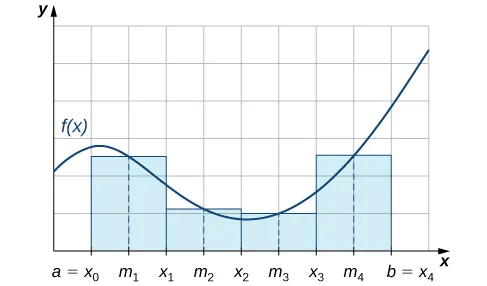
\includegraphics[scale=0.5]{figures/pic1.png }
    \end{center}     
     \end{minipage}

     \pagebreak \bigbreak \noindent 
     \begin{eg}[Using the midpoint rule with $M_{4}$]
         Use the midpoint rule to estimate  $\int_{0}^{1}\ x^{2}\ dx $ using four subintervals. Compare the result with the actual value of this integral.
     \end{eg}
      \bigbreak \noindent 
      \textbf{Solution:} Each subinterval has a length of $\Delta x = \frac{b-a}{n} = \frac{1}{4}$. Thus we have the partition 
         \begin{align*}
             P=\bigg\{0,\frac{1}{4},\frac{1}{2}, \frac{3}{4}, 1\bigg\}\ \quad \text{(Normal partition)}
         .\end{align*}
         \bigbreak \noindent 
         To find the midpoints between each interval, we can divide $\Delta x$ by 2. Thus we have 
         \begin{align*}
             P = \bigg\{\frac{1}{8}, \frac{3}{8},\frac{5}{8}, \frac{7}{8}\bigg\}
         .\end{align*}
         \bigbreak \noindent 
         With:
         \begin{align*}
             &S = \bigg\{f\left(\frac{1}{8}\right), f\left(\frac{3}{8}\right), f\left(\frac{5}{8}\right), f\left(\frac{7}{8}\right)\bigg\} \\
             &=\bigg\{\frac{1}{64}, \frac{9}{64}, \frac{25}{64}, \frac{49}{64}, \bigg\}
         .\end{align*}
         \bigbreak \noindent 
         From this we can compute:
         \begin{align*}
             &M_{4} = \summation{n}{i=1}\ f(m_{i})\Delta x \\
             &= \frac{1}{4}\bigg[\frac{1}{64}+\frac{9}{64}+\frac{25}{64} + \frac{49}{64}\bigg] \\
             &= \frac{21}{64}
         .\end{align*}
         \bigbreak \noindent 
         Know, because the function $x^{2}$ is an elementary function, we can find the actual antiderivative and compute the error in our estimate.
         \begin{align*}
             &\int_{0}^{1}\ x^{2}\ dx \\
             &=\frac{1}{3}
         .\end{align*}
         \bigbreak \noindent 
         Thus the error is: 
         \begin{align*}
             &\bigg|\frac{1}{3}-\frac{21}{64}\bigg| \\
             &=\frac{1}{921} \approx 0.0052
         .\end{align*}
         we see that the midpoint rule produces an estimate that is somewhat close to the actual value of the definite integral.

         \pagebreak \bigbreak \noindent 
         \phantomsection
         \addcontentsline{toc}{subsection}{The Trapezoidal Rule}
         \subsection*{The Trapezoidal Rule}
         \bigbreak \noindent 
         \begin{minipage}[t]{0.47\textwidth}
             We can also approximate the value of a definite integral by using trapezoids rather than rectangles. In Figure 3.14, the area beneath the curve is approximated by trapezoids rather than by rectangles.
         \end{minipage}
         \begin{minipage}[]{0.47\textwidth}
            \bigbreak \noindent 
            \begin{center}
                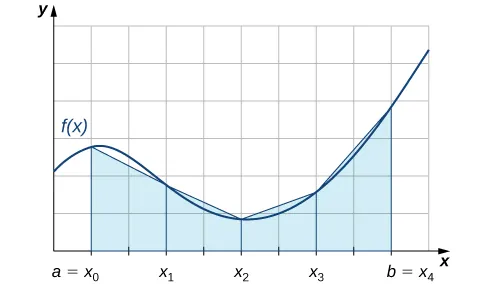
\includegraphics[scale=0.5]{./figures/pic2.png}
            \end{center}
         \end{minipage}
         \bigbreak \noindent 
         The trapezoidal rule for estimating definite integrals uses trapezoids rather than rectangles to approximate the area under a curve. To gain insight into the final form of the rule, consider the trapezoids shown in Figure 3.14. We assume that the length of each subinterval is given by $\Delta x$.
        First, recall that the area of a trapezoid with a height of $h$ and bases of length $b_1$ and $b_2$ is given by $\text{Area} = \frac{1}{2} h (b_1 + b_2)$.
        We see that the first trapezoid has a height $\Delta x$ and parallel bases of length $f(x_0)$ and $f(x_1)$. Thus, the area of the first trapezoid in Figure 3.14 is
        \begin{align*}
            \frac{1}{2}\Delta x(f(x_{0}) + f(x_{1}))
        .\end{align*}
        The areas of the remaining three trapezoids are
        \[
            \frac{1}{2} \Delta x (f(x_1) + f(x_2)), \frac{1}{2} \Delta x (f(x_2) + f(x_3)), \text{and} \frac{1}{2} \Delta x (f(x_3) + f(x_4)).
        \]
        Consequently,
        \[
        \int_a^b f(x) \, dx \approx \frac{1}{2} \Delta x (f(x_0) + f(x_1)) + \frac{1}{2} \Delta x (f(x_1) + f(x_2)) + \frac{1}{2} \Delta x (f(x_2) + f(x_3)) + \frac{1}{2} \Delta x (f(x_3) + f(x_4)).
        \]
        After taking out a common factor of $\frac{1}{2} \Delta x$ and combining like terms, we have
        \[
        \int_a^b f(x) \, dx \approx \frac{1}{2} \Delta x \left( f(x_0) + 2f(x_1) + 2f(x_2) + 2f(x_3) + f(x_4) \right).
        \]
        Generalizing, we formally state the following rule.
        \bigbreak \noindent 
        \begin{thrm}[The Trapezoidal Rule]
            Assume that $f(x)$ is continuous over $[a,b]$.
            Let $n$ be a positive integer and $\Delta x = \frac{b-a}{n}$.
            Let $[a,b]$ be divided into $n$ subintervals, each of length $\Delta x$, 
            with endpoints at $P = \{ x_0, x_1, x_2, \ldots, x_n \}$.
            Set:
            \begin{align*}
                &T_n = \frac{1}{2} \Delta x \left( f(x_0) + 2f(x_1) + 2f(x_2) + \cdots + 2f(x_{n-1}) + f(x_n) \right). 
            .\end{align*}
            Then $\lim_{{n \to +\infty}} T_n = \int_a^b f(x) \, dx$
        \end{thrm}

        \pagebreak \bigbreak \noindent 
        Before continuing, let’s make a few observations about the trapezoidal rule. First of all, it is useful to note that
        \begin{align*}
            &T_n = \frac{1}{2} (L_n + R_n)\ \text{where}\ L_n = \sum_{i=1}^{n} f(x_{i-1}) \Delta x\ \text{and}\ R_n = \sum_{i=1}^{n} f(x_i) \Delta x
        .\end{align*}
        \bigbreak \noindent 
        That is, $L_{n}$ and  $R_{n}$ approximate the integral using the left-hand and right-hand endpoints of each subinterval, respectively. In addition, a careful examination of Figure 3.15 leads us to make the following observations about using the trapezoidal rules and midpoint rules to estimate the definite integral of a nonnegative function. The trapezoidal rule tends to overestimate the value of a definite integral systematically over intervals where the function is concave up and to underestimate the value of a definite integral systematically over intervals where the function is concave down. On the other hand, the midpoint rule tends to average out these errors somewhat by partially overestimating and partially underestimating the value of the definite integral over these same types of intervals. This leads us to hypothesize that, in general, the midpoint rule tends to be more accurate than the trapezoidal rule.

        \bigbreak \noindent 
        \phantomsection
        \addcontentsline{toc}{subsection}{Absolute and Relative Error}
        \subsection*{Absolute and Relative Error}
        \bigbreak \noindent 
        An important aspect of using these numerical approximation rules consists of calculating the error in using them for estimating the value of a definite integral. We first need to define \textbf{absolute error} and \textbf{relative error}.
        \bigbreak \noindent 
        If $B$ is our estimate of some quantity having an actual value of $A$,  then the absolute error is given by $|A-B|$. The relative error is the error as a percentage of the absolute value and is given by 
        \[
        \left| \frac{A-B}{A} \right| = \left| \frac{A-B}{A} \right| \cdot 100\%.
        \]
        \bigbreak \noindent 
        Although, it is quite obvious that we do not typically have the luxury of knowing the actual value. In general, if we are approximating an integral, we are doing so because we cannot compute the exact value of the integral itself easily. Therefore, it is often helpful to be able to determine an upper bound for the error in an approximation of an integral. The following theorem provides error bounds for the midpoint and trapezoidal rules. The theorem is stated without proof.
        \bigbreak \noindent 
        \begin{thrm}[Error Bounds for the Midpoint and Trapezoidal Rules]
            Let $f(x)$ be a continuous function over $[a,b]$, having a second derivative $f''(x)$ over this interval. If $M$ is the maximum value of $|f''(x)|$ over $[a,b]$, then the upper bounds for the error in using $M_n$ and $T_n$ to
            \bigbreak \noindent 
            Estimate $\int_{a}^{b}\ \ dx $ are:
            \begin{align*}
                E_{M} = \frac{M(b-a)^{3}}{24n^{2}}
            .\end{align*}
            And:
            \begin{align*}
                E_{T} = \frac{M(b-a)^{3}}{12n^{2}}
            .\end{align*}
        \end{thrm}
        \bigbreak \noindent 
        We can use these bounds to determine the value of $n$ necessary to guarantee that the error in an estimate is less than a specified value.

        \pagebreak \bigbreak \noindent 
        \begin{eg}[Determining the Number of Intervals to Use]
            What value of  $n$ should be used to guarantee that an estimate of  $\int_{0}^{1}\ e^{x^{2}}\ dx $ is accurate to within 0.01 if we use the midpoint rule?
        \end{eg}
        \bigbreak \noindent 
        \textbf{Solution:}
        We begin by determining the value of $M$,  the maximum value of $|f^{\prime\prime}(x)|$ over $[0,1]$  for $f(x) = e^{x^2}$.  Since $f^{\prime}(x) = 2x e^{x^2}$,  we have:
        \begin{align*}
            f^{\prime\prime}(x) = 2e^{x^2} + 4x^2 e^{x^2}.
        .\end{align*}
        Thus:
        \begin{align*}
            f^{\prime\prime}(x) = 2e^{x^2} + 4x^2 e^{x^2}.
        .\end{align*}
        From the error-bound Equation \(3.12\), we have
        \[
            \text{Error in } M_n \leq \frac{M(b-a)^3}{24n^2} \leq \frac{6e(1-0)^3}{24n^2} = \frac{6e}{24n^2}.
        \]
        \bigbreak \noindent 
        Now we solve the following inequality for  $n$:
        \begin{align*}
            \frac{6e}{24n^{2}} \leq 0.01
        .\end{align*}
        Thus, \( n \geq \sqrt{\frac{600e}{24}} \approx 8.24 \). Since \( n \) must be an integer satisfying this inequality, a choice of \( n=9 \) would guarantee that \( \left| \int_0^1 e^{x^2} dx - M_n \right| < 0.01 \).

        \bigbreak \noindent 
        \textbf{Analysis}
        \bigbreak \noindent 
        We might have been tempted to round 8.24 down and choose $n=8 $, but this would be incorrect because we must have an integer greater than or equal to 8.24. We need to keep in mind that the error estimates provide an upper bound only for the error. The actual estimate may, in fact, be a much better approximation than is indicated by the error bound.

        \bigbreak \noindent 
        \phantomsection
        \addcontentsline{toc}{subsection}{Simpson’s Rule}
        \subsection*{Simpson’s Rule}
        \bigbreak \noindent 
        With the midpoint rule, we estimated areas of regions under curves by using rectangles. In a sense, we approximated the curve with piecewise constant functions. With the trapezoidal rule, we approximated the curve by using piecewise linear functions. What if we were, instead, to approximate a curve using piecewise quadratic functions? With Simpson’s rule, we do just this. We partition the interval into an even number of subintervals, each
        of equal width. Over the first pair of subintervals we approximate $\int_{x_0}^{x_2} f(x) \, dx$ with $\int_{x_0}^{x_2} p(x) \, dx$, where $p(x) = Ax^2 + Bx + C$ is the quadratic function passing through $(x_0, f(x_0))$, $(x_1, f(x_1))$, and $(x_2, f(x_2))$ (Figure 3.16). Over the next pair of subintervals we approximate $\int_{x_2}^{x_4} f(x) \, dx$ with the integral of another quadratic function passing through $(x_2, f(x_2))$, $(x_3, f(x_3))$, and $(x_4, f(x_4))$. This process is continued with each successive pair of subintervals.
        \bigbreak \noindent 
        \begin{center}
            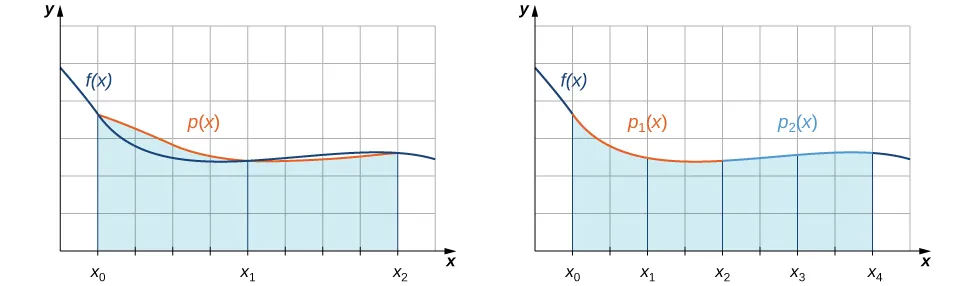
\includegraphics[scale=0.5]{./figures/mane1.png}
        \end{center}

        \pagebreak \bigbreak \noindent 
        To understand the formula that we obtain for Simpson’s rule, we begin by deriving a formula for this approximation over the first two subintervals. As we go through the derivation, we need to keep in mind the following relationships:
        \begin{align*}
            f(x_0) &= p(x_0) &= Ax_0^2 + Bx_0 + C \\
            f(x_1) &= p(x_1) &= Ax_1^2 + Bx_1 + C \\
            f(x_2) &= p(x_2) &= Ax_2^2 + Bx_2 + C
        .\end{align*}
        $x_2 - x_0 = 2 \Delta x$, where $\Delta x $ is the length of a subinterval
        \begin{align*}
            x_{2} + x_{0} = 2x_{1},\ \text{since}\ x_{1} = \frac{(x_{2} + x_{0})}{2}
        .\end{align*}
        Thus:
        \begin{align*}
            \int_{x_0}^{x_2} f(x) \, dx &\approx \int_{x_0}^{x_2} p(x) \, dx \\
            &= \int_{x_0}^{x_2} (Ax^2 + Bx + C) \, dx \\
            &= \left[ \frac{A}{3}x^3 + \frac{B}{2}x^2 + Cx \right]_{x_0}^{x_2}\ \quad \text{(Find the antiderivative)} \\
            &=\frac{A}{3}(x_{2}^{3}-x_{0}^{3}) + \frac{B}{2}(X_{2}^{2}-x_{0}^{2})+C(x_{2}-x_{0}) \quad \text{(Evaluate the antiderivative)} \\
            &=\frac{A}{3}(x_{2}-x_{0})(x_{2}^{2}+x_{2}x_{0}+x_{0}^{2}) \\
            &+\frac{B}{2}(x_{2}-x_{0})(x_{2}+x_{0})+  C(x_{2}-x_{0}) \\
            &=\frac{x_{2}-x_{0}}{6}(2A(x_{2}^{2}+x_{2}x_{0}+x_{0}^{2})) + 3B(x_{2} +x_{0} + 6C) \quad \text{(Factor out $\frac{x_{2}-x_{0}}{6} $)} \\
            &=\frac{\Delta x}{3}((Ax_{2}^{2} + Bx_{2} + C) +(Ax_{0}^{2}+Bx_{0}+ C)) \\
            &+A(x_{2}td2)+2x_{2}x_{0}+x_{0}^{2}) + 2B(x_{2}+x_{0} + 4C) \\
            &=\frac{\Delta x}{3}(f(x_{2})+f(x_{0})+A(x_{2}+x_{0})^{2}+2B(x_{2}+x_{0}) + 4C) \quad \text{(Rearrange the terms)} \\
            &=\frac{\Delta x}{3}(f(x_{2})+f(x_{0})+A(2x_{1})^{2}+2B(2x_{1})+4C) \quad \text{(Substitute $x_{2} + x_{0}  = 2x_{1}$)} \\
            &=\frac{\Delta x}{3}(f(x_{2})+4f(x_{1}) +f(x_{0})) \quad \text{(Expand and substitute $f(x_{1}) = Ax_{1}^{2} + Bx_{1} + C$)}
        \end{align*}
        \bigbreak \noindent 
        If we approximate $\int_{x_{2}}^{x_{4}}\ f(x)\ dx $ using the same method, we see that we have:
        \begin{align*}
            \int_{x_{2}}^{x_{4}}\ f(x)\ dx \approx \frac{\Delta x}{3}(f(x_{4}) +4f(x_{3}) + f(x_{2}))
        .\end{align*}
        \bigbreak \noindent 
        Combining these two approximations we get:
        \begin{align*}
            \int_{x_{0}}^{x_{4}}\ f(x)\ dx = \frac{\Delta x}{3}(f(x_{0}) +4f(_{1}) +2f(x_{2})+4f(x_{3})+f(x_{4}))
        .\end{align*}
        \bigbreak \noindent 
        The pattern continues as we add pairs of subintervals to our approximation. The general rule may be stated as follows.
        \pagebreak \bigbreak \noindent 
        \begin{thrm}[Simpson’s Rule]
            Assume that $f(x)$ is continuous over $[a,b]$. Let $n$ be a positive even integer and $\Delta x = \frac{b-a}{n}$. Let $[a,b]$ be divided into $n$ subintervals, each of length $\Delta x$, with endpoints at $P=\{x_0, x_1, x_2, \dots, x_n\}$. Set
            \begin{align*}
                S_n = \frac{\Delta x}{3} \left( f(x_0) + 4f(x_1) + 2f(x_2) + 4f(x_3) + 2f(x_4) + 4f(x_5) + \cdots + 2f(x_{n-2}) + 4f(x_{n-1}) + f(x_n) \right)
            .\end{align*}
            Then:
            \begin{align*}
                \lim\limits_{n \to +\infty}{S_{n} = \int_{a}^{b}\ f(x)\ dx}
            .\end{align*}
        \end{thrm}
        \bigbreak \noindent 
        Just as the trapezoidal rule is the average of the left-hand and right-hand rules for estimating definite integrals, Simpson’s rule may be obtained from the midpoint and trapezoidal rules by using a weighted average. It can be shown that $S_{2n} = \frac{2}{3}M_{n} + \frac{1}{3}T_{n}$
        \bigbreak \noindent 
        It is also possible to put a bound on the error when using Simpson’s rule to approximate a definite integral. The bound in the error is given by the following rule:
        \bigbreak \noindent 
        \begin{thrm}[Error bound for Simpson's rule]
           Let $f(x)$ be a continuous function over $[a,b]$ having a fourth derivative, $f^{(4)}(x)$, over this interval. If $M$ is the maximum value of $|f^{(4)}(x)|$ over $[a,b]$, then the upper bound for the error in using $S_n$ to estimate
           \smallbreak \noindent
           $\int_{a}^{b}\ f(x)\ dx $ is given by:
           \begin{align*}
               E_{S} \leq \frac{M(b-a)^{5}}{180n^{4}}
           .\end{align*}
        \end{thrm}

        \pagebreak \bigbreak \noindent 
        \phantomsection
        \addcontentsline{toc}{section}{3.7 Improper Integrals}
        \section*{3.7 Improper Integrals}
        \bigbreak \noindent 
        


        







        
        


        






\end{document}
